\documentclass[12pt]{article}

\usepackage[margin=1.0in]{geometry}
\usepackage{graphicx}
\usepackage{listings}
\usepackage{tabto}
\usepackage{multicol}
\usepackage{lipsum}
\usepackage{caption}
\usepackage{mwe}
\usepackage{tikz}
\usepackage{tabto}
\usetikzlibrary{automata,positioning}
\usepackage{enumitem}
\usepackage{amsmath}
\usepackage{amssymb}
\graphicspath{ {./} }


\begin{document}

\title{CS4347 : Database Systems\\Homework Assignment 7}
\author{Matthew McMillianmgm160130@utdallas.edu}
\maketitle



\begin{enumerate}

	\item[14.19)] Suppose that we have the following requirements for a university database that is used to keep track of students’ transcripts: First show all the functional dependencies
that should hold among the attributes. Then design relation schemas for the database that are each in 3NF or BCNF. Specify the key attributes of each relation. Note any unspecified requirements, and make appropriate assumptions to render the specification complete.
	\begin{center}
			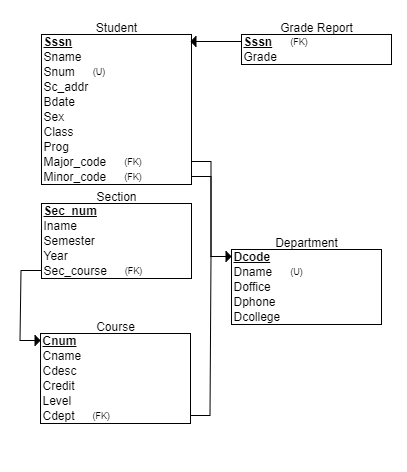
\includegraphics[scale=1]{hw7r1}
	\end{center} 
		\textbf{Functional Dependencies:} \\
		Sssn $\rightarrow$ Sname, Bdate, Sex\\
		Sname $\rightarrow$ Sc$\_$addr\\
		Snum $\rightarrow$ Major$\_$code, Class, Minor$\_$code, Prog\\
		Dcode $\rightarrow$ Dname, Doffice, Dphone, Dcollege\\
		Cnum $\rightarrow$ Cname, Cdept, Credit, Level\\
		Cname $\rightarrow$ Cdesc \\ \\
		Above, a relation in 3rd normal form. Ssn defines a person's identity, such as name, bdate, and sex. However Ssn doesn't define someone's address, which is variable to lots of change unlike name, sex, bdate. Student number is related to the university's side of things, and it implies information about their person at the university such as Major/Minor and progress information. Department code is descriptive of the name, location, phone/office, and college information. Cnum represents a specific course and gives information about that course, but the Cname is the factor that describes a course, and its description should be related to the course name. Some additional information that would be useful is if Cdept was referring to the department name or code. Also It would be helpful to know if Sec$\_$course referred to a Cname or a Cnum. \\
		
	\item[14.20)] What update anomalies occur in the EMP$\_$PROJ and EMP$\_$DEPT relations of Figures 14.3 and 14.4? \\ \\
	Possible update anomalies could occur when rows are inserted or deleted, or when updating a value on a related table (i.e. updating EMP$\_$Dept or EMP$\_$Proj). Some trivial things to be aware of are incomplete updates (though there should be contingencies to avoid this). Other anomalies such as update anomalies include updating Pname(s) and Dname(s), or insert anomalies based on constraints, and deletion anomalies based on constraints. (For example, if project requires at least 1 employee, insert and deletions of projects would invalidate certain rows). \\
	
	\item[14.21)]  In what normal form is the LOTS relation schema in Figure 14.12(a) with respect to the restrictive interpretations of normal form that take only the primary key into account? Would it be in the same normal form if the general definitions of normal form were used? \\ \\
	The current schema in 14.12(a) is in 1st normal form. If you take away the restrictive interpretation, we can normalize into (and up to according to the figure) 4th normal form. Therefore, if we restrict our our definition to just a primary key, we see that we have a hard time normalizing.
	\pagebreak
	
	\item[14.29)] Consider the following relations for an order-processing application database at ABC, Inc. ORDER (O$\#$, Odate, Cust$\#$, Total$\_$amount) ORDER$\_$ITEM(O$\#$, I$\#$, Qty$\_$ordered, Total$\_$price, Discount$\%$) Assume that each item has a different discount. The Total$\_$price refers to one item, Odate is the date on which the order was placed, and the Total$\_$amount is the amount of the order. If we apply a natural join on the relations ORDER$\_$ITEM and ORDER in this database, what does the resulting relation schema look like? What will be its key? Show the FDs in this resulting relation. Is it in 2NF? Is it in 3NF? Why or why not? (State assumptions, if you make any.) \\ \\
	Below is the resulting table if we natural join order and order$\_$item
	
	\begin{center}
			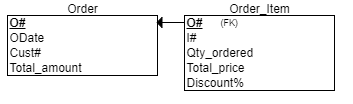
\includegraphics[scale=1]{hw7r2} \\
			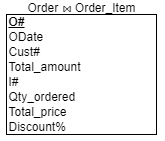
\includegraphics[scale=1]{hw7r3}
	\end{center}
	
	\textbf{Functional Dependencies:} \\
	O$\#$ $\rightarrow$ Total$\_$amount, Odate, Qty$\_$ordered \\
	I$\#$ $\rightarrow$ Total$\_$price, Discount$\%$ \\

	The relation (not the naturally joined table) is in 2nd normal form since we are in 1st normal form, and since all the columns of both functional dependencies are dependent on that relation's primary key and the key only. This is not in 3rd normal form (and inductively any other form above 3) since we do not have an transitive relational properties within this table. \\
	\pagebreak
	
	\item[14.35)] BOOK (Book$\_$Name, Author, Edition, Year) with the data: a. Based on a common-sense understanding of the above data, what are the possible candidate keys of this relation? b. Justify that this relation has the MVD $\{$ Book $\}$ $\rightarrow \rightarrow$ $\{$ Author $\}$ $|$ $\{$ Edition, Year $\}$. c. What would be the decomposition of this relation based on the above MVD? Evaluate each resulting relation for the highest normal form it possesses. \\ \\
	\begin{itemize}
		\item[a.] Author could be a candidate key since it is uniquely descriptive of a set of books. Book could also be a possible candidate key since it also has some uniquely defining factors. Edition and Year are both very broad, and they don't have much uniqueness to themselves so they may not be an optional choice for a candidate key.
		\item[b.] Edition and Year do not have any dependencies among eachother, so we can have these as part of a MVD. A book implies an author, since one or more authors wrote a book. Also a book can imply multiple editions and years (which are linked together loosely). Thus, it makes sense to form a MVD here.
		\item[c.] We could convert this to 2nd normal form by forming the tables below:
		\begin{center}
			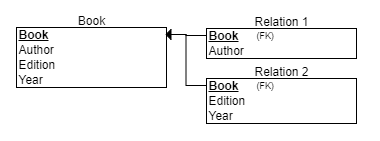
\includegraphics[scale=1]{hw7r4}
		\end{center}
		However after some rearranging of the relation, we could convert to 3rd normal form:
		\begin{center}
			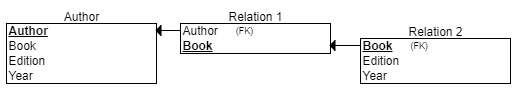
\includegraphics[scale=1]{hw7r5}
		\end{center}
	\end{itemize}
	\pagebreak
	\item[14.36]  Consider the following relation: TRIP (Trip$\_$id, Start$\_$date, Cities$\_$visited, Cards$\_$used) This relation refers to business trips made by company salespeople. Suppose the TRIP has a single Start$\_$date, but involves many Cities and salespeople may use multiple credit cards on the trip. Make up a mock-up population of the table. a. Discuss what FDs and/or MVDs exist in this relation. b. Show how you will go about normalizing it.
	\begin{itemize}
		\item[a.]
	\textbf{Multi-Valued Dependencies:} \\	
	$\{$Trip$\_$id$\}$ $\rightarrow$ $\rightarrow$ $\{$ Cities$\_$visited, Cards$\_$used$\}$\\
	
	\textbf{Functional Dependencies:} \\
	$\{$Trip$\_$id$\}$ $\rightarrow$ $\{$ Start$\_$date $\}$\\
	Here, the multiple value dependencies and the functional dependencies differ slightly. It would be nice to have more information, but the cities and cards used seem to be independent of the tripid, and they can be combined into a MVD. For the functional dependencies, the start date is directly related to the trip$\_$id.
	
	\item[b.] We would have to convert this into three relations, resulting in a normalization in 2nd normal form since the columns of the table are not dependent on each other. 
		\begin{center}
			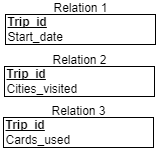
\includegraphics[scale=1]{hw7r6}
		\end{center}
	
	\end{itemize}

	
\end{enumerate}


\end{document}
